\documentclass[conference]{IEEEtran}
\IEEEoverridecommandlockouts

\usepackage{cite}
\usepackage{amsmath,amssymb,amsfonts}
\usepackage{graphicx}
\usepackage{booktabs}
\usepackage{url}

\renewcommand{\arraystretch}{0.95}
\setlength{\textfloatsep}{6pt plus 1pt minus 2pt}
\setlength{\intextsep}{6pt plus 1pt minus 2pt}
\setlength{\abovecaptionskip}{2pt}
\setlength{\belowcaptionskip}{0pt}

\begin{document}

\title{When Does Text Help? A Leakage-Free Information-Richness and
Encoder-Adaptation Study for Multimodal Land-Cover Composition Regression\\
{\large DI 725 Final Report (Phase 3)}}

\author{\IEEEauthorblockN{\"Omer Faruk Merey}
\IEEEauthorblockA{Graduate School of Informatics, Middle East Technical University \\
omer.merey@metu.edu.tr}}

\maketitle

\begin{abstract}
We study whether auxiliary text captions improve land-cover composition
regression from satellite imagery on ARAS400k, under strict no-leakage
conditions. The dataset's hybrid captions embed the ground-truth percentages
verbatim, so we restrict text to the leakage-free vision-only captions and add
numeric sanitization. We evaluate an information-richness axis (empty caption,
no-text floor, keywords, two qualitative captions, random text) with frozen
CLIP encoders, then introduce the project's principal ablation: unfreezing the
encoder via LoRA. Three results emerge. (1) With frozen encoders, the
cross-attention block --- not the text --- drives the gain, and clean captions
help only when they correctly describe the image (a fidelity-conditional effect
that averages near zero). (2) LoRA fine-tuning lowers test MSE by 32--60\,\%
and \emph{reverses the architectural story}: once the encoder adapts, the
pure-vision model becomes the best and the fusion layer no longer helps.
(3) A controlled leakage condition (raw hybrid captions) collapses MSE to
$\sim$1/5 of the best leakage-free model, quantifying the failure mode that
motivated the redesign.
\end{abstract}

\begin{IEEEkeywords}
remote sensing, land cover, multimodal learning, CLIP, cross-attention,
LoRA, data leakage, ablation
\end{IEEEkeywords}

%-------------------------------------------------------------------------
\section{Introduction}

Land-cover composition is a structured regression target: seven mutually
exclusive classes (Tree, Shrub, Grass, Crop, Built-up, Barren, Water) summing
to 100\,\%. ARAS400k~\cite{aras400k} provides 10\,000 RGB tiles, segmentation
masks, and five caption variants generated by vision-language models (VLMs).
The project asks whether captions improve composition regression beyond a
vision-only baseline, and if so by how much.

The original design was found to contain a structural \textbf{data-leakage}
path: the \texttt{hybrid\_*} and \texttt{text\_qwen3-4b} captions state the
ground-truth percentages verbatim (e.g.\ ``grasslands~(92\,\%)''). A model
trained against them solves the task lexically rather than multimodally.
Crucially, the leak is not merely lexical: the VLMs that wrote those captions
saw the percentages, so even stripping the digits leaves a label-shaped
narrative. We therefore restrict text to the two \texttt{vision\_*} captions
(generated from the image alone) and apply numeric sanitization as a safety
filter.

\textbf{Research question.} \emph{How does the semantic richness of auxiliary
text captions --- from a vision-only baseline, to keywords, to detailed
qualitative descriptions --- impact land-cover composition regression while
strictly avoiding data leakage, and how does this change when the visual
encoder is allowed to adapt?}

\textbf{Contributions.}
(1)~A leakage-free information-richness ablation with frozen encoders, plus a
random-text control and a caption-fidelity stratified evaluation.
(2)~A LoRA encoder-adaptation ablation that severely changes the results and
reverses the frozen-regime conclusion about the fusion layer.
(3)~A controlled leakage condition that quantifies, rather than merely asserts,
the leakage failure mode.

%-------------------------------------------------------------------------
\section{Related Work}

CLIP~\cite{clip} aligns image and text via contrastive pretraining; its
adaptation to remote sensing is studied in RemoteCLIP~\cite{remoteclip} and
RS5M~\cite{rs5m}, which report that domain adaptation of the encoder is the
dominant lever for downstream gains --- consistent with our LoRA findings.
Cross-attention fusion has been shown to outperform late fusion in
remote-sensing segmentation~\cite{ftransunet}; we find that this advantage is
contingent on the encoder being frozen. Parameter-efficient fine-tuning via
low-rank adapters~\cite{lora} lets us adapt a frozen CLIP cheaply, which is
what turns the architectural story around in Section~\ref{sec:disc}.

%-------------------------------------------------------------------------
\section{Methodology}

\subsection{Architecture}
A frozen CLIP ViT-B/32 encodes the image into 49 patch tokens and the caption
into 77 token embeddings. An 8-head cross-attention block uses image patches as
queries and text tokens as keys/values; the 49 fused vectors are mean-pooled
and passed to a \texttt{Linear}(512$\to$256)$\to$\texttt{ReLU}$\to$\texttt{Linear}(256$\to$7)$\to$\texttt{Softmax}
head. Loss is MSE on the softmax output against the target distribution. The
pure-vision variant removes cross-attention (patches $\to$ mean-pool $\to$
head).

\subsection{Conditions}
The information-richness axis is realised by six frozen conditions plus a
random-text control (Table~\ref{tab:conditions}); numbers in all text are
masked to a \texttt{[NUM]} placeholder to prevent residual leakage. R1 keywords
are noun lemmas extracted with spaCy over both \texttt{vision\_*} captions and
are deliberately \emph{not} filtered to the target classes, which would inject
GT structure. A caption-fidelity stratified test additionally tags each test
tile \texttt{agree}/\texttt{disagree} by whether a synonym of the dominant GT
class appears in the conditioning caption.

\begin{table}[t]
\centering\footnotesize
\caption{Conditions. CA = cross-attention; GAP = patch mean-pool.}
\label{tab:conditions}
\begin{tabular}{@{}lll@{}}
\toprule
\textbf{Code} & \textbf{Arch.} & \textbf{Text input} \\
\midrule
R0a    & CLIP+CA+MLP  & empty token \\
R0b    & CLIP+GAP+MLP & --- (no text) \\
R1     & CLIP+CA+MLP  & noun-lemma keywords (both \texttt{vision\_*}) \\
R2a    & CLIP+CA+MLP  & sanitized \texttt{vision\_gemma3-4b} \\
R2b    & CLIP+CA+MLP  & sanitized \texttt{vision\_qwen3-vl-8b} \\
R-rand & CLIP+CA+MLP  & 77 random vocab tokens (control) \\
\midrule
\multicolumn{3}{@{}l}{\emph{Phase 3 additions}}\\
*-lora & + LoRA on encoder & R0a/R0b/R2b, encoder unfrozen \\
Rleak  & CLIP+CA+MLP & raw \texttt{hybrid\_gemma3-4b} (GT \%, leaky) \\
\bottomrule
\end{tabular}
\end{table}

\subsection{LoRA encoder adaptation (principal ablation)}
The severe change is unfreezing CLIP via low-rank adapters. We inject
LoRA ($r{=}8$, $\alpha{=}16$) into the MLP projections of the last six
residual blocks of both encoders; the packed-QKV attention projection is left
untouched because \texttt{nn.MultiheadAttention} bypasses its module forward.
Only the adapters, the cross-attention block, and the head are trained
($\sim$1.4\,M parameters); the CLIP base stays frozen. We fine-tune in fp32 and
apply gradient clipping (max-norm 1.0), which removed a divergence observed for
the empty-caption (R0a) condition --- the lowest-signal case for the fusion
layer. We re-train R0a, R0b, and R2b with LoRA and compare against their frozen
counterparts.

\subsection{Leakage quantification}
\texttt{Rleak} trains on the raw, unsanitized \texttt{hybrid\_gemma3-4b}
caption (percentages intact) as a controlled negative control --- a failure
mode to measure, not a method to advocate.

\subsection{Training and reproducibility}
AdamW (lr $10^{-4}$ frozen, $5\!\times\!10^{-5}$ LoRA, weight decay $10^{-4}$),
cosine annealing, early stopping, deterministic 70/15/15 split, three seeds per
condition. Because frozen CLIP outputs are constant across epochs, frozen runs
read precomputed fp16 embeddings (the full frozen grid runs in under an hour on
an Apple M4); LoRA runs are online ($\sim$84\,s/epoch on the same machine).
Runs are tracked on Weights \& Biases.

%-------------------------------------------------------------------------
\section{Results}

\subsection{Frozen regime}
Table~\ref{tab:frozen} and Fig.~\ref{fig:frozen} give the frozen-encoder test
MSE. Removing cross-attention (R0b) is by far the largest effect; among
caption-bearing conditions the empty caption (R0a) is numerically best, and
the empty caption significantly beats random text
($p{=}8.6\!\times\!10^{-9}$), so caption content is not irrelevant but is
dominated by other factors. The fidelity-stratified test
(Table~\ref{tab:fidelity}) shows why captions look unhelpful on average: R2a/R2b
match or beat R0a on tiles whose caption mentions the dominant class, and
underperform by a comparable margin when it does not.

\begin{table}[t]
\centering\footnotesize
\caption{Frozen-encoder test MSE/MAE, mean $\pm$ std over 3 seeds.}
\label{tab:frozen}
\setlength{\tabcolsep}{4pt}
\begin{tabular}{@{}lcc@{}}
\toprule
\textbf{Cond.} & \textbf{MSE} $\downarrow$ & \textbf{MAE} $\downarrow$ \\
\midrule
R0a    & \textbf{.00707}$\pm$.00006 & \textbf{.0406}$\pm$.0003 \\
R0b    & .01101$\pm$.00032 & .0554$\pm$.0011 \\
R1     & .00760$\pm$.00016 & .0425$\pm$.0008 \\
R2a    & .00751$\pm$.00026 & .0422$\pm$.0009 \\
R2b    & .00739$\pm$.00020 & .0421$\pm$.0007 \\
R-rand & .00787$\pm$.00008 & .0425$\pm$.0002 \\
\bottomrule
\end{tabular}
\end{table}

\begin{table}[t]
\centering\footnotesize
\caption{Caption-fidelity stratified test MSE (frozen).}
\label{tab:fidelity}
\begin{tabular}{@{}lcc@{}}
\toprule
\textbf{Cond.} & \textbf{MSE (agree)} & \textbf{MSE (disagree)} \\
\midrule
R0a & .00676 & .00740 \\
R2a & \textbf{.00671} & .00823 \\
R2b & .00680 & .00787 \\
\bottomrule
\end{tabular}
\end{table}

\subsection{LoRA regime (principal ablation)}
Table~\ref{tab:lora} and Fig.~\ref{fig:lora} report the frozen-vs-LoRA
comparison. LoRA lowers MSE by 32--60\,\% on every condition. The ordering
\emph{flips}: in the frozen regime R0a (cross-attention) far outperforms R0b
(pure vision); under LoRA the pure-vision R0b becomes the best condition, and
the cross-attention conditions no longer help.

\begin{table}[t]
\centering\footnotesize
\caption{Frozen vs.\ LoRA test MSE (mean over 3 seeds) and relative change.}
\label{tab:lora}
\setlength{\tabcolsep}{5pt}
\begin{tabular}{@{}lccc@{}}
\toprule
\textbf{Cond.} & \textbf{Frozen} & \textbf{LoRA} & \textbf{$\Delta$} \\
\midrule
R0a & .00707 & .00478$\pm$.0001 & $-$32\,\% \\
R0b & .01101 & \textbf{.00435}$\pm$.0001 & $-$60\,\% \\
R2b & .00739 & .00466$\pm$.0002 & $-$37\,\% \\
\bottomrule
\end{tabular}
\end{table}

\begin{figure}[t]
\centering
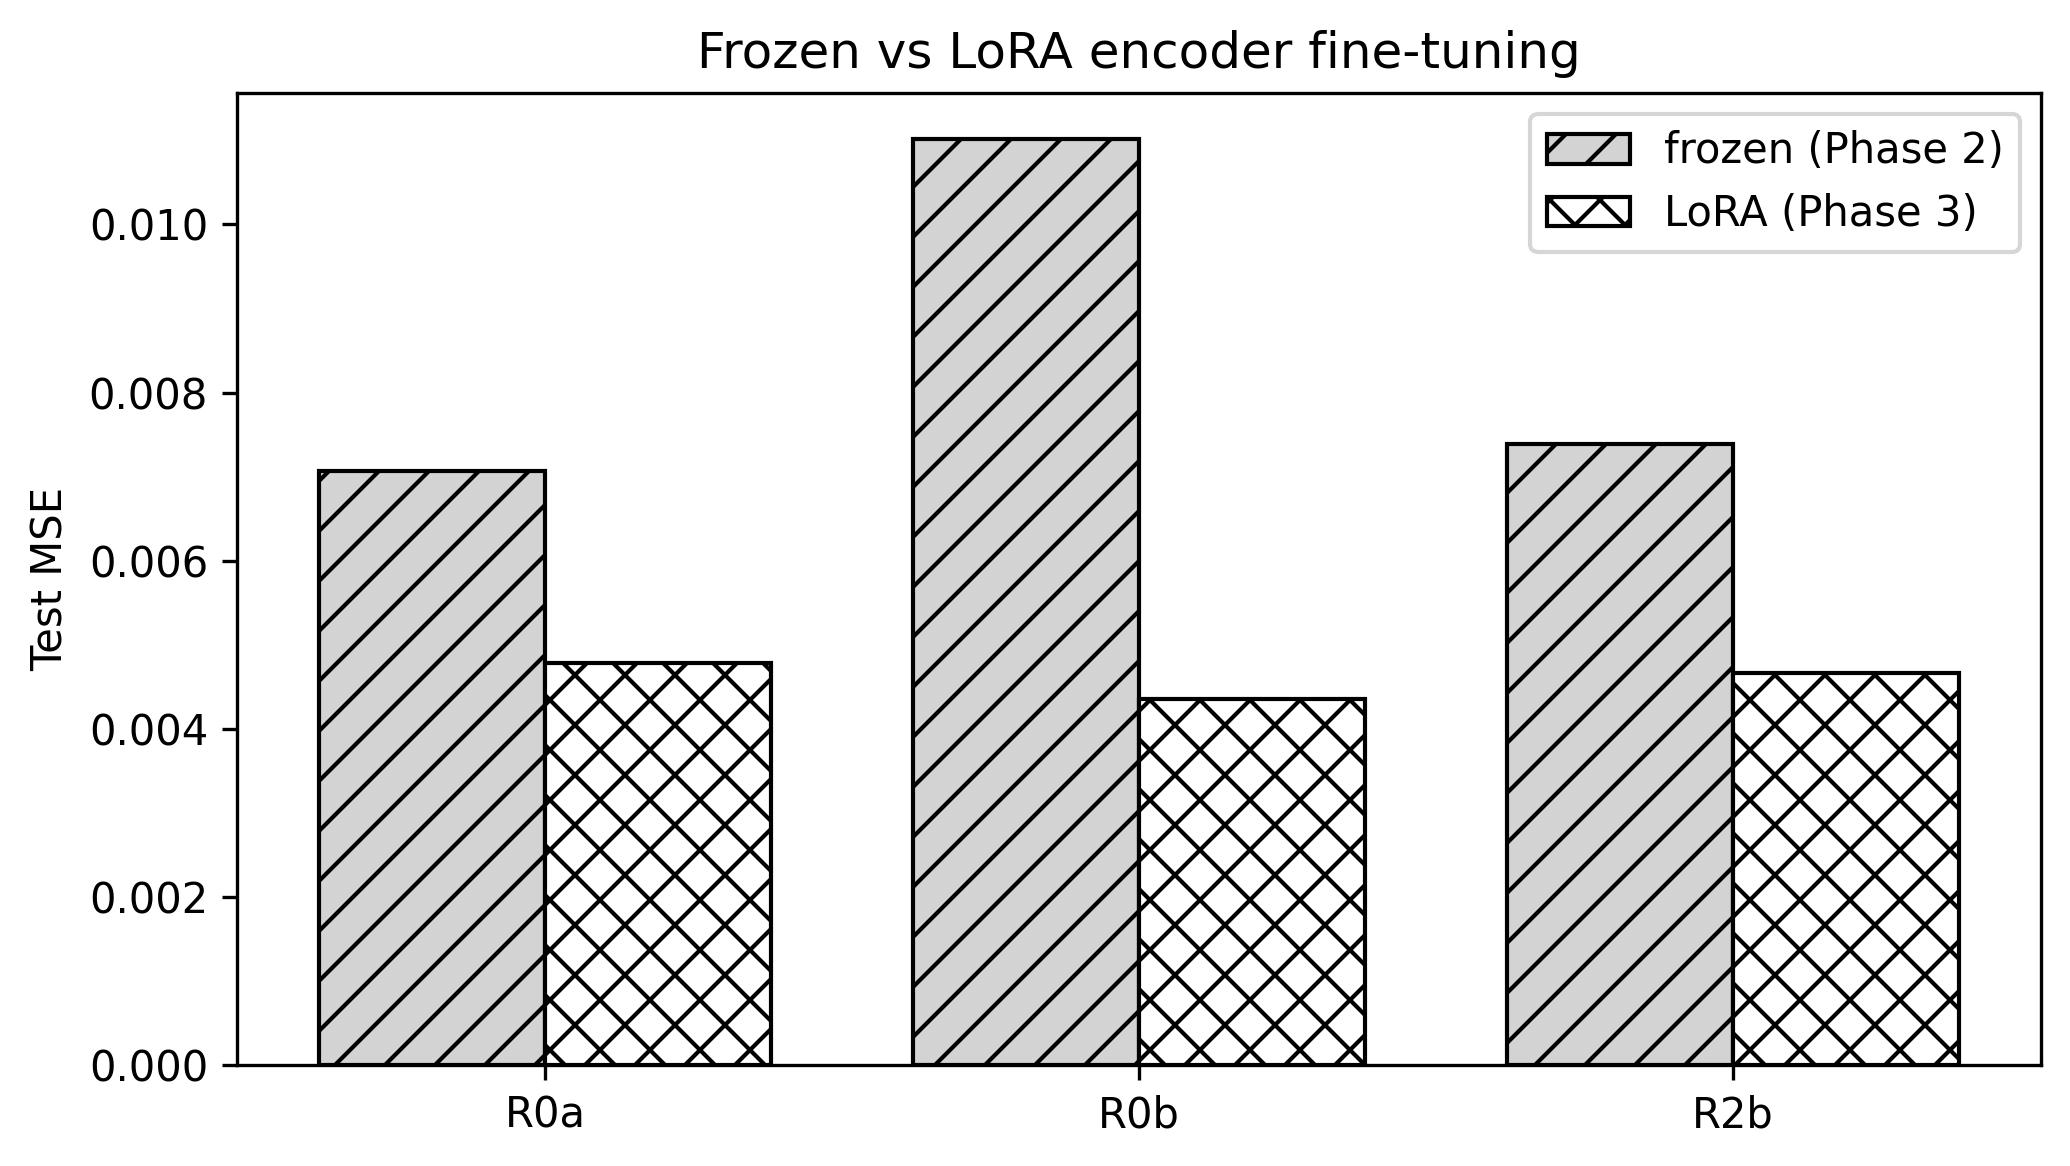
\includegraphics[width=0.86\linewidth]{phase3_frozen_vs_lora.png}
\caption{Frozen vs.\ LoRA test MSE. LoRA improves all conditions; the
pure-vision R0b benefits most and becomes the best model.}
\label{fig:lora}
\end{figure}

\subsection{Leakage quantification}
\texttt{Rleak} attains test MSE $0.00143\pm0.0001$ --- about one third of the
best leakage-free model (R0b-lora, $0.00435$) and one fifth of the frozen R0a
baseline (Fig.~\ref{fig:leak}). The model recovers the targets almost directly
from the percentages in the text.

\begin{figure}[t]
\centering
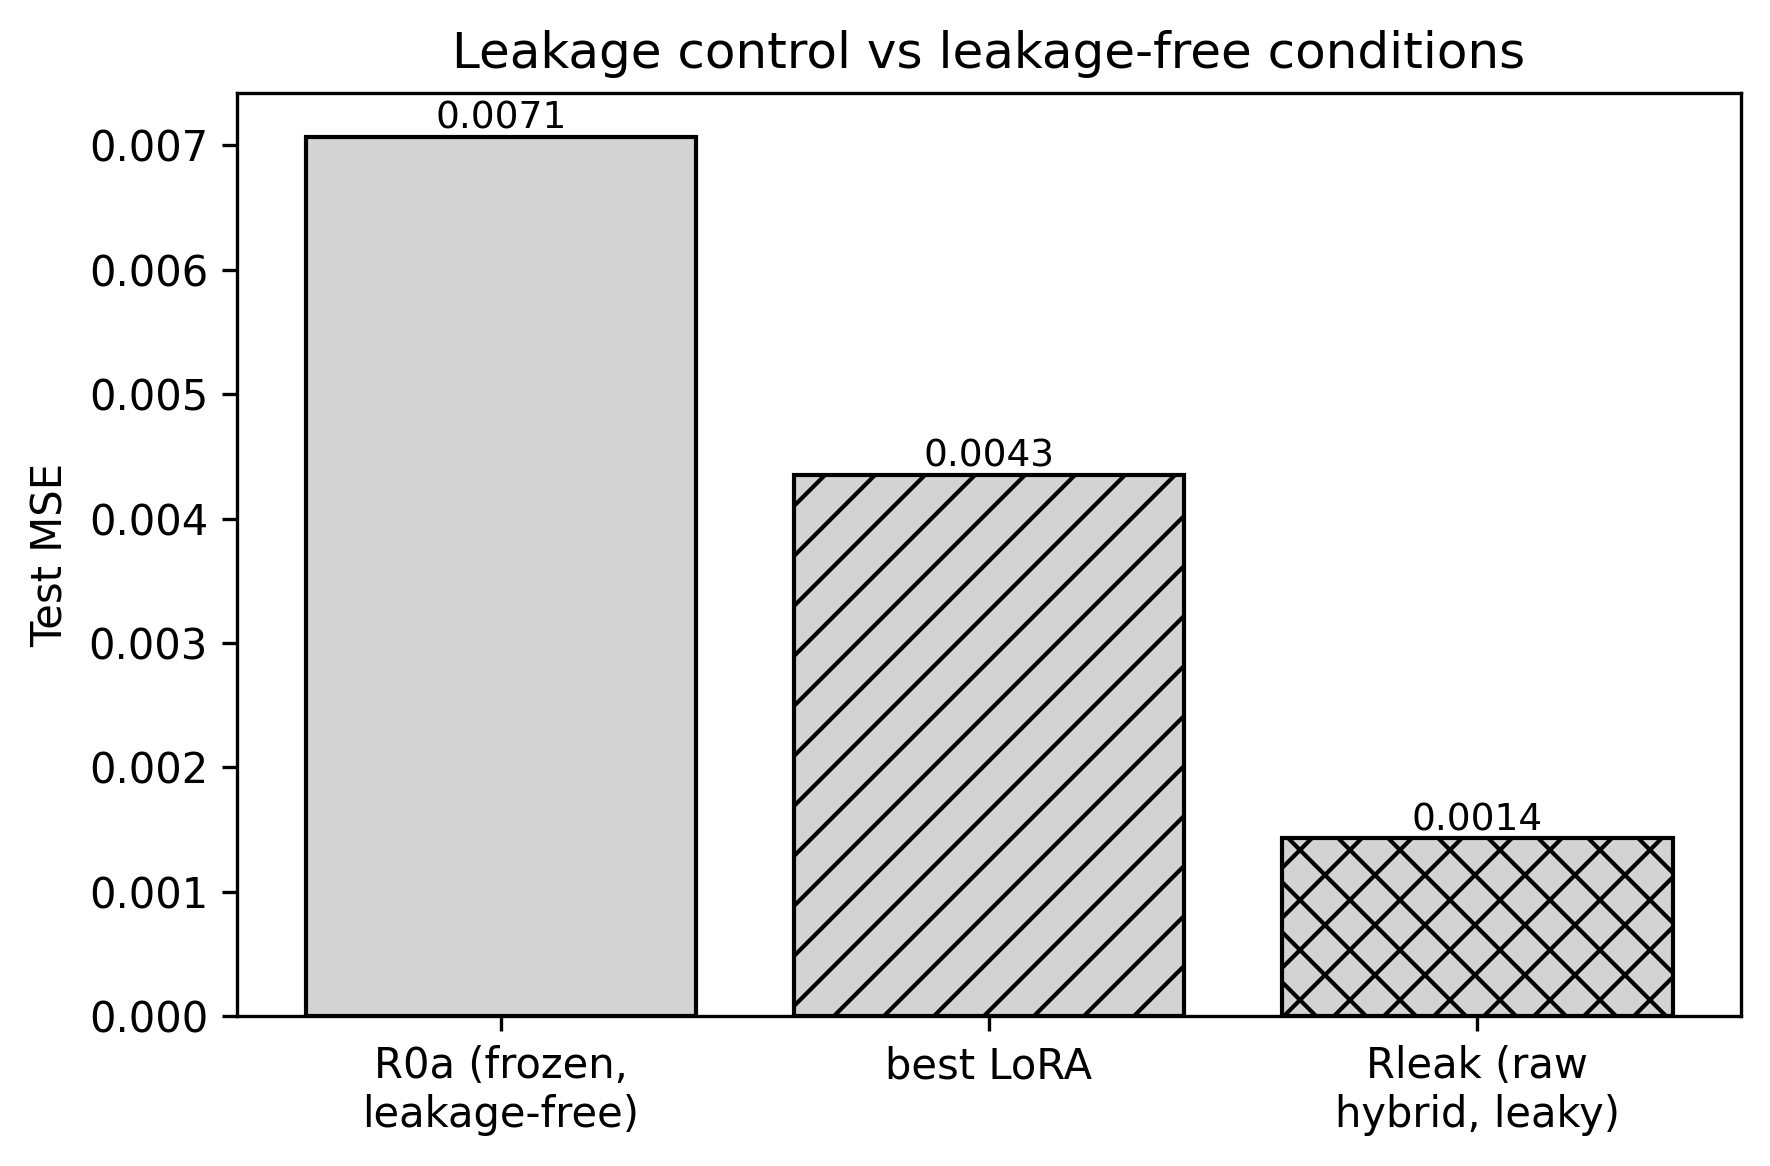
\includegraphics[width=0.74\linewidth]{phase3_leakage.png}
\caption{Leakage control. \texttt{Rleak} (raw hybrid, GT \% in text) collapses
MSE far below the leakage-free conditions.}
\label{fig:leak}
\end{figure}

\begin{figure}[t]
\centering

\includegraphics[width=0.86\linewidth]{phase2_mse_bar_with_rrand.png}
\caption{Frozen-regime information-richness ablation (incl.\ R-rand control).}
\label{fig:frozen}
\end{figure}

%-------------------------------------------------------------------------
\section{Discussion}
\label{sec:disc}

\textbf{Frozen regime: architecture, not text.} The dominant frozen effect is
architectural --- the cross-attention block, even with an empty caption, gives
a $\sim$36\,\% lower MSE than the pure-vision floor. Without an
architecture-matched no-text baseline (R0b) this would have been miscredited to
the text. Clean captions provide only a fidelity-conditional benefit
(Table~\ref{tab:fidelity}) that cancels on average, and noun keywords are
statistically indistinguishable from random text. ``Adding captions'' is thus
not a uniform intervention: fidelity, not richness, gates the effect.

\textbf{Encoder adaptation reverses the story.} The principal ablation shows
that the frozen-regime conclusion is regime-dependent. Once LoRA lets the
visual encoder adapt, the pure-vision model (R0b-lora, $0.00435$) overtakes the
cross-attention conditions (R0a-lora $0.00478$, R2b-lora $0.00466$): the fusion
layer's contribution in the frozen regime was effectively a capacity
substitute for a non-adapted encoder, and it becomes redundant --- even mildly
harmful over an empty/degenerate text path --- once the encoder itself can
learn. This aligns with RemoteCLIP/RS5M~\cite{remoteclip,rs5m}, where encoder
domain-adaptation is the dominant lever, and qualifies the cross-attention
advantage reported for frozen fusion in~\cite{ftransunet}. The caption signal
remains marginal in both regimes (R2b-lora edges R0a-lora by $\sim$2.5\,\%).

\textbf{Leakage, quantified.} \texttt{Rleak} makes the Phase-1 concern concrete:
percentage-bearing captions yield an MSE $3$--$5\times$ lower than any
leakage-free model, an ``improvement'' that reflects text copying rather than
multimodal reasoning. This is the quantitative justification for excluding
hybrid captions throughout.

\textbf{Limitations.} A single \texttt{synth} domain; LoRA on MLP projections
only (attention QKV untouched); the fidelity tag is a lexical proxy; the
empty-caption LoRA condition required gradient clipping for stability.

%-------------------------------------------------------------------------
\section{Conclusion}

Under leakage-free conditions, multimodal gains on ARAS400k are dominated by
the visual pathway, not the text. With frozen encoders the cross-attention
fusion block carries the apparent ``multimodal'' improvement and clean captions
help only conditionally on their fidelity to the image; with a LoRA-adapted
encoder the pure-vision model is best and the fusion layer becomes redundant.
A controlled leakage condition confirms that percentage-bearing captions
produce large but illusory gains. Methodologically, multimodal claims must be
ablated against architecture-matched no-text, random-text, and
encoder-adaptation baselines before any non-trivial text contribution is
asserted.

%-------------------------------------------------------------------------
\section*{Reproducibility}
Code, notebooks with outputs, and \texttt{requirements.txt}:
\url{https://github.com/OmerFarukMerey/remote-sensing-caption-composition}.
W\&B: \url{https://wandb.ai/mereyomerfaruk/di725-project}.

\begin{thebibliography}{6}
\bibitem{clip} A.~Radford \emph{et al.}, ``Learning transferable visual models
from natural language supervision,'' in \emph{Proc.\ ICML}, 2021,
pp.~8748--8763.
\bibitem{remoteclip} F.~Liu \emph{et al.}, ``RemoteCLIP: A vision language
foundation model for remote sensing,'' \emph{IEEE Trans.\ Geosci.\ Remote
Sens.}, vol.~62, pp.~1--16, 2024.
\bibitem{rs5m} Z.~Zhang \emph{et al.}, ``RS5M and GeoRSCLIP: A large scale
vision-language dataset and model for remote sensing,'' \emph{IEEE Trans.\
Geosci.\ Remote Sens.}, vol.~62, pp.~1--23, 2024.
\bibitem{ftransunet} X.~Ma, X.~Zhang, M.-O.~Pun, and M.~Liu, ``A multilevel
multimodal fusion transformer for remote sensing semantic segmentation,''
\emph{IEEE Trans.\ Geosci.\ Remote Sens.}, vol.~62, pp.~1--15, 2024.
\bibitem{lora} E.~J.~Hu \emph{et al.}, ``LoRA: Low-rank adaptation of large
language models,'' in \emph{Proc.\ ICLR}, 2022.
\bibitem{aras400k} M.~\c{C}a\u{g}lar, ``ARAS400k Remote Sensing Dataset,''
Zenodo, 2026. [Online]. Available: \url{https://zenodo.org/records/18890661}
\end{thebibliography}

\end{document}
